\appendix
\chapter{Allgemeines}

\newpage

\section{Zeitplan}

\begin{figure} [H]
	\begin{center}
		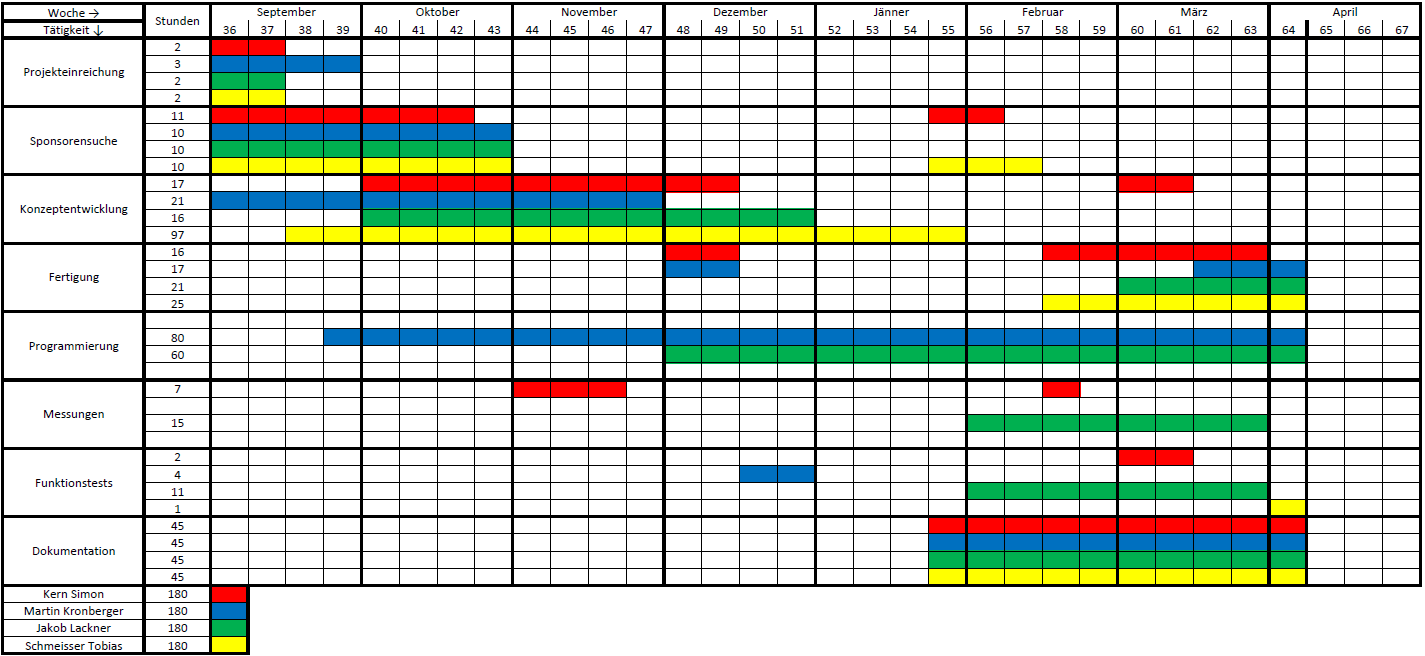
\includegraphics[angle=90, scale=0.6] {figures/allgemein/zeitplan.png}
		\caption{Zeitplan und Arbeitszeiten}
		\label{fig:Zeitplan}
	\end{center}
\end{figure}

\newpage

\section{Kosten}


\begin{figure} [H]
	\begin{center}
		\includegraphics[angle=-90, scale=0.6] {figures/allgemein/stückliste.png}
		\caption{Kostenaufstellung und Stückliste}
		\label{fig:Stückliste}
	\end{center}
\end{figure}

\newpage

\chapter{Programmcode}



\chapter{CAD-Zeichnungen}

\newpage

\section{Mechanik}

\begin{figure} [H]
	\begin{center}
		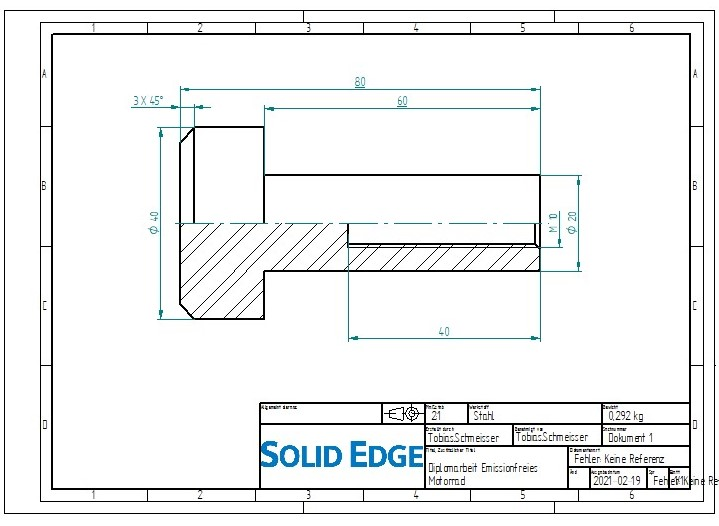
\includegraphics[angle=90, scale=0.9] {figures/mechanik/Welle_Rechts_Zeichnung.jpg}
		\caption{Wellenersatz}
		\label{fig:Wellenersatz1}
	\end{center}
\end{figure}

\fancyfoot[C]{Schmeisser}

\newpage

\begin{figure} [H]
	\begin{center}
		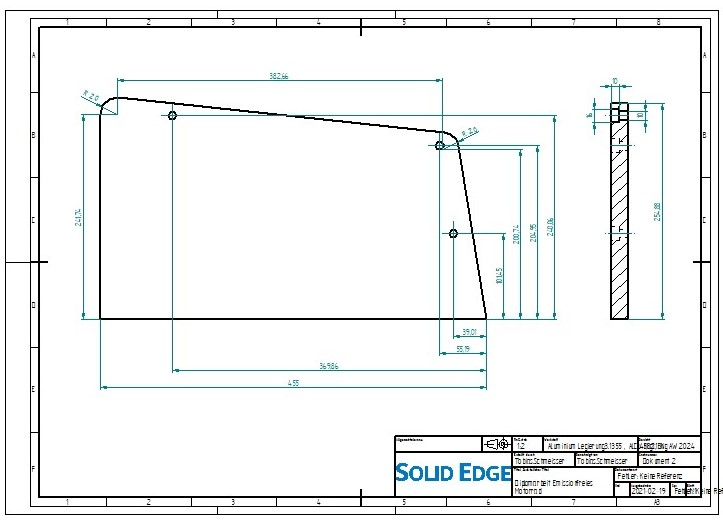
\includegraphics[angle=90]{figures/mechanik/Seitenplatte_Fertigung_Rechts.jpg}
		\caption{Seitenplatte Rechts}
		\label{fig:SeitenplatteRechts}
	\end{center}
\end{figure}


\begin{figure} [H]
	\begin{center}
		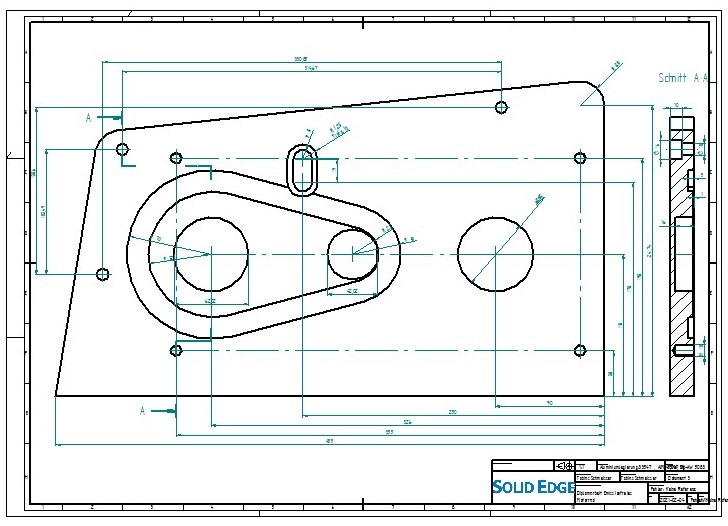
\includegraphics[angle=90]{figures/mechanik/Seitenplatte_Fertigung_Links.jpg}
		\caption{Seitenplatte Links}
		\label{fig:Seitenplatte Links}
	\end{center}
\end{figure}


\begin{figure} [H]
	\begin{center}
		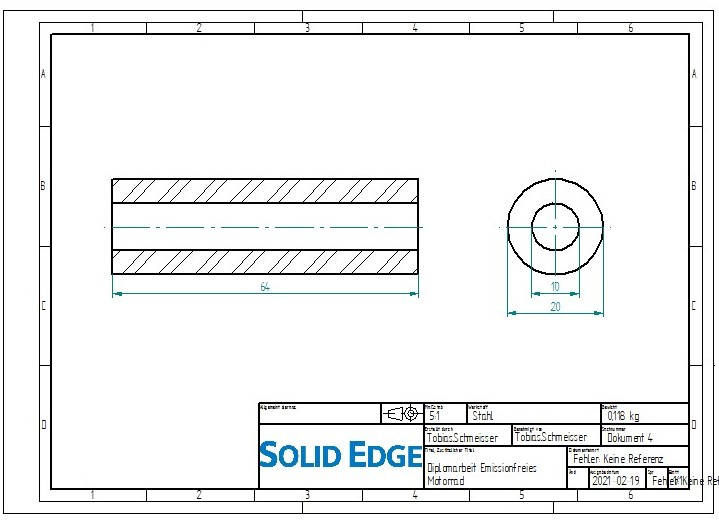
\includegraphics[angle=90]{figures/mechanik/Seitenplatte_Abstandhalter_Zeichnung.jpg}
		\caption{Abstandhalter}
		\label{fig:Abstandhalter}
	\end{center}
\end{figure}


\begin{figure} [H]
	\begin{center}
		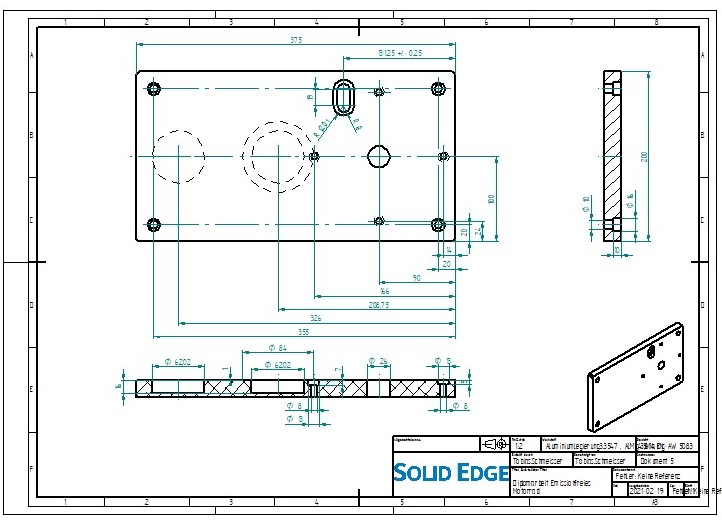
\includegraphics[angle=90]{figures/mechanik/Aufbau_Seitenplatte_Links_Zeichn.jpg}
		\caption{Aufbau/Zusatzplatte}
		\label{fig:Aufbau/Zusatzplatte}
	\end{center}
\end{figure}


\begin{figure} [H]
	\begin{center}
		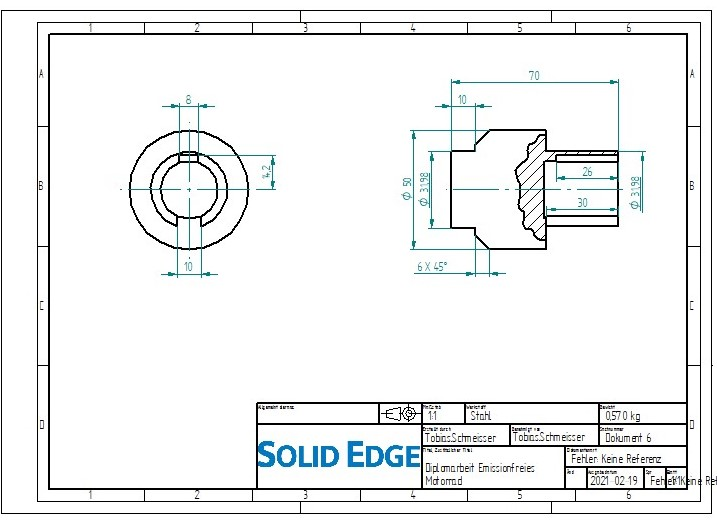
\includegraphics[angle=90]{figures/mechanik/Antriebsachse_Zeichnung.jpg}
		\caption{Achse 1/Antriebsachsen}
		\label{fig:Achse 1/Antriebsachsen}
	\end{center}
\end{figure}


\begin{figure} [H]
	\begin{center}
		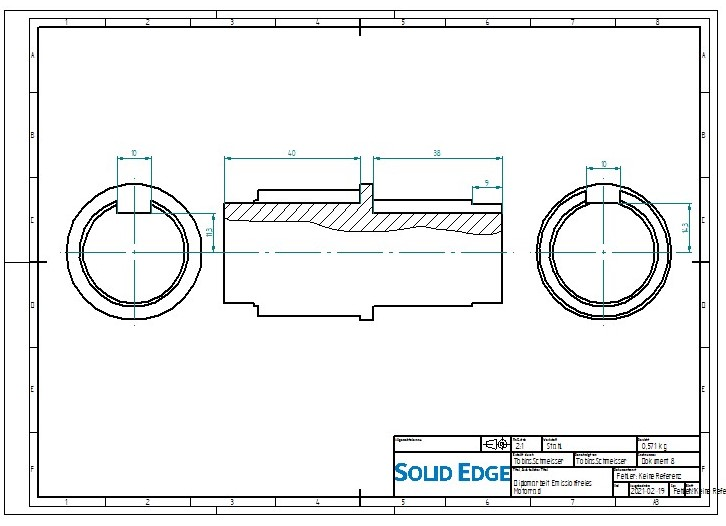
\includegraphics[angle=90]{figures/mechanik/Achse_mit_nuten_Zeichnung.jpg}
		\caption{Achse 3}
		\label{fig:Achse3}
	\end{center}
\end{figure}


\begin{figure} [H]
	\begin{center}
		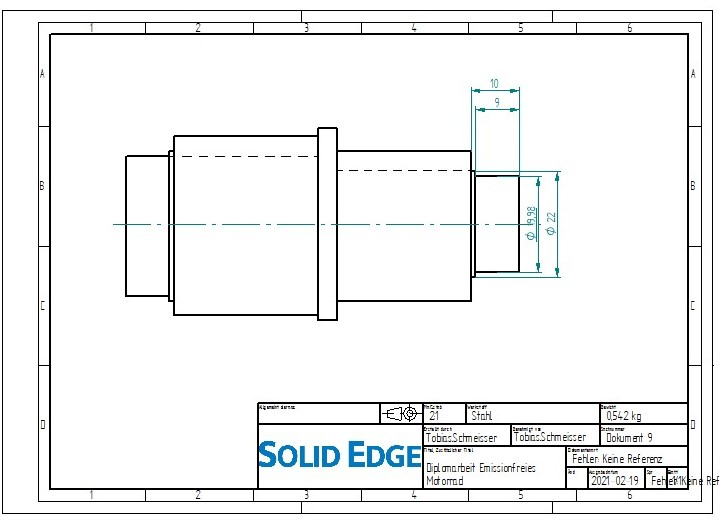
\includegraphics[angle=90]{figures/mechanik/Achse_mit_nuten_20mm_Zeichnung.jpg}
		\caption{Achse 2}
		\label{fig:Achse2}
	\end{center}
\end{figure}


\begin{figure} [H]
	\begin{center}
		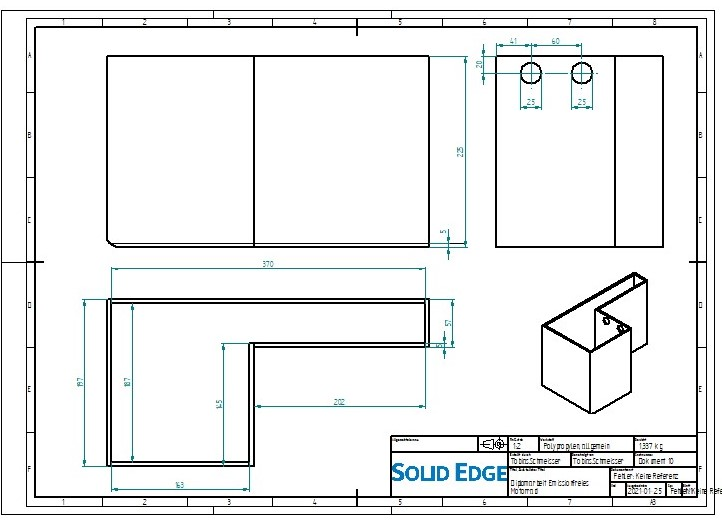
\includegraphics[angle=90]{figures/mechanik/Box_Zeichnung.jpg}
		\caption{Akkubox Motorblock}
		\label{fig:Akkubox Motorblock}
	\end{center}
\end{figure}


\begin{figure} [H]
	\begin{center}
		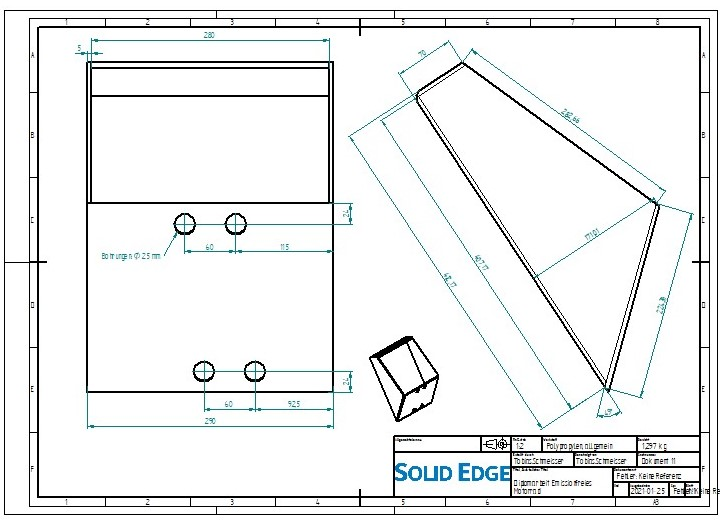
\includegraphics[angle=90]{figures/mechanik/Box_2_Zeichnung.jpg}
		\caption{Akkubox Vorderseite}
		\label{fig:Akkubox Vorderseite}
	\end{center}
\end{figure}


\begin{figure} [H]
	\begin{center}
		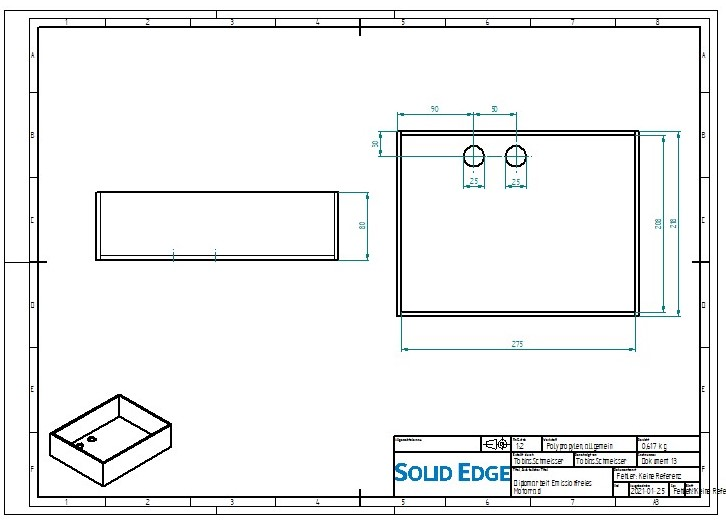
\includegraphics[angle=90]{figures/mechanik/Box_3_Zeichnung.jpg}
		\caption{Akkubox Mitte}
		\label{fig:Akkubox Mitte}
	\end{center}
\end{figure}

\section{HCIS} \label{app:hcis}



\begin{figure} [H]
	\begin{center}
		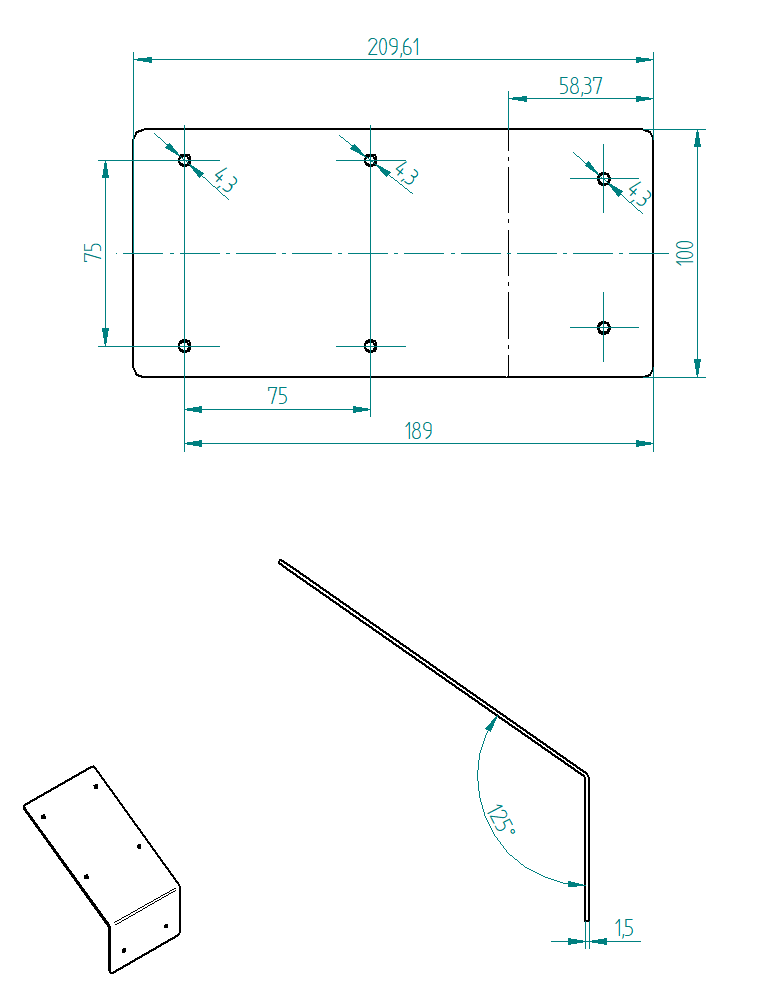
\includegraphics[scale=0.8]{figures/hcis/befestigung_display_cad.png}
		\caption{Akkubox Mitte}
		\label{fig:panel_cad}
	\end{center}
\end{figure}

\fancyfoot[C]{Kronberger}

\chapter{Simulationen}

\section{Mechanik}

\fancyfoot[C]{Schmeisser}


\includepdf[pages=-, pagecommand={\thispagestyle{fancy}}, scale=0.95] {figures/mechanik/Simulationen/Seitenplatte_Links_Statische Berechnung 1_3.pdf}

\includepdf[pages=-, pagecommand={\thispagestyle{fancy}}, scale=0.95] {figures/mechanik/Simulationen/Seitenplatte_Rechts_Statische Berechnung 1_3.pdf}

\chapter{Schaltpläne}

\fancyfoot[C]{Kronberger}

\newpage

\section{HCIS}




\chapter{Datenblätter}


\fancyfoot[C]{Kronberger}

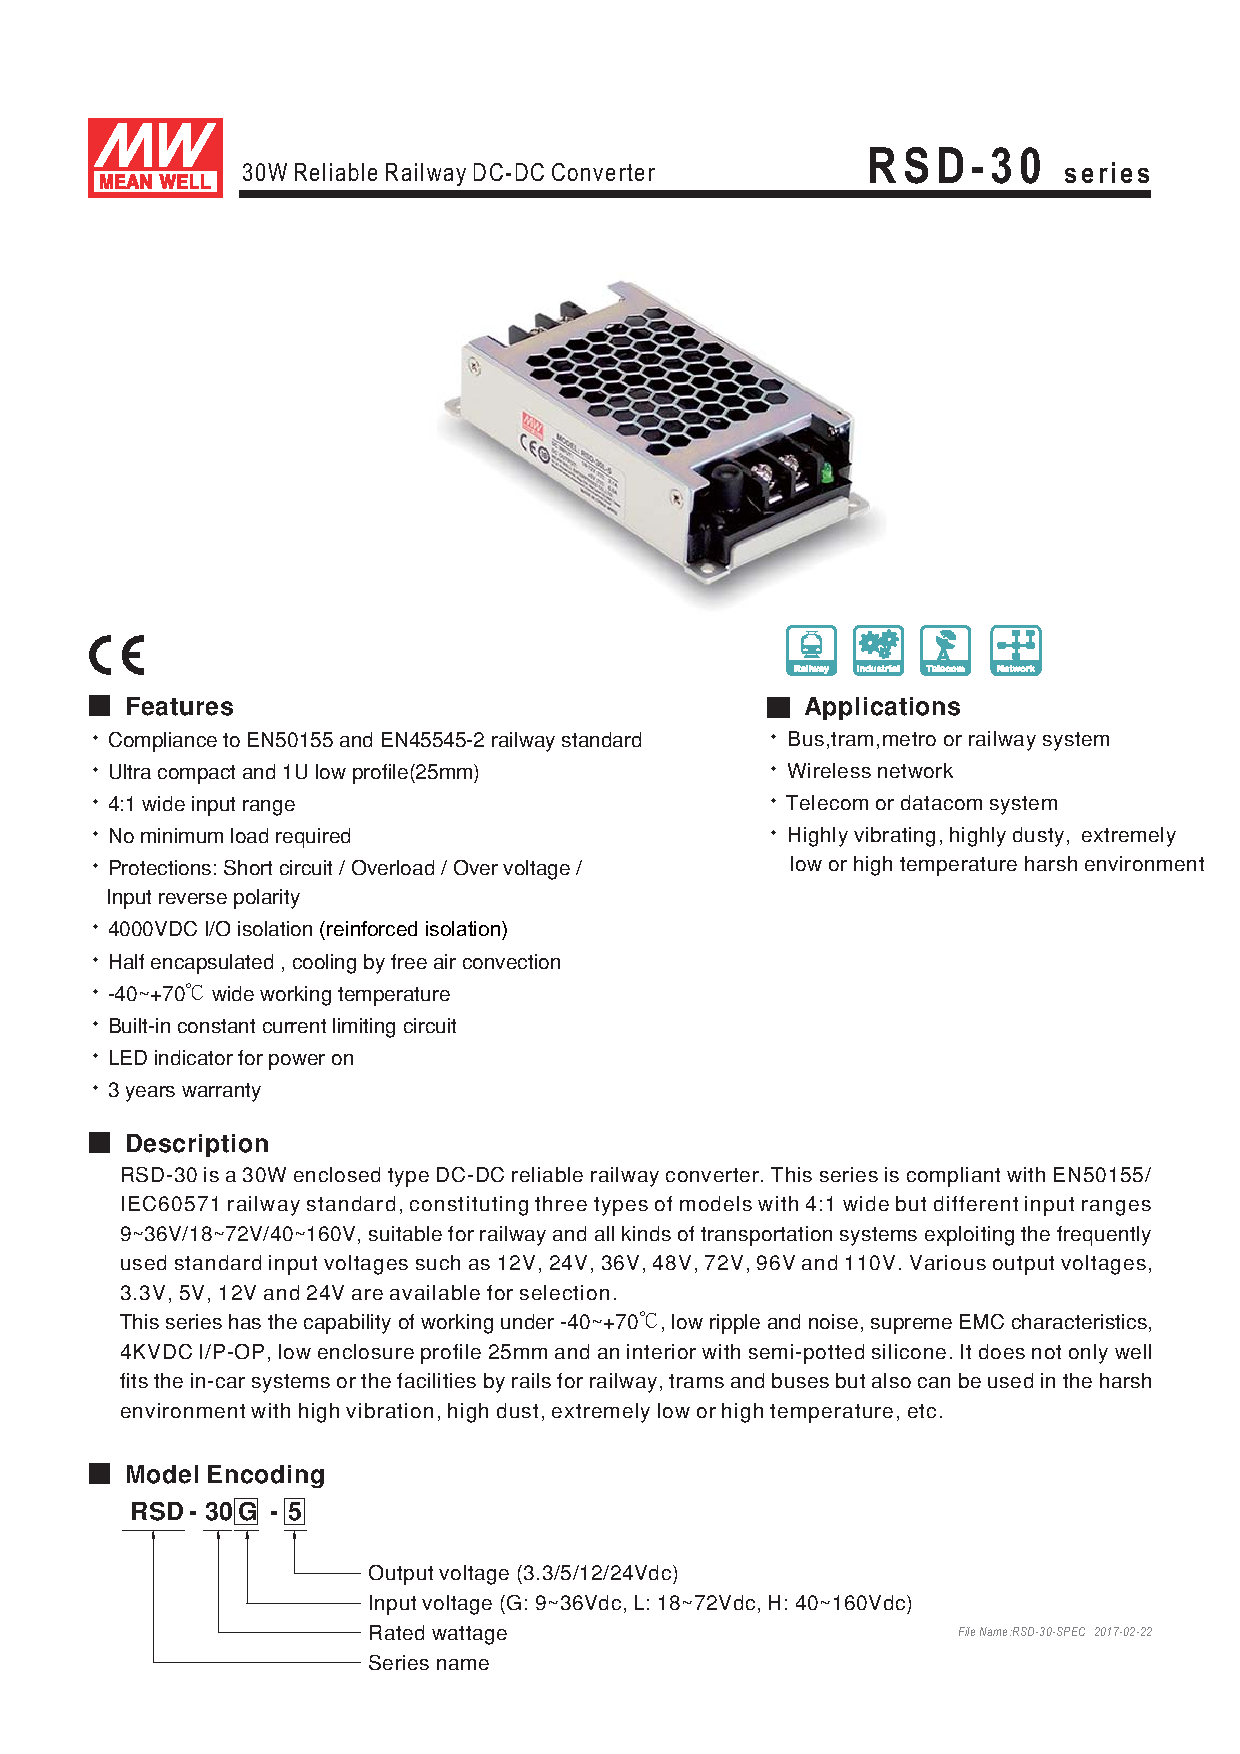
\includepdf[pages=1, pagecommand={\thispagestyle{fancy}}, pagecommand={\section{HCIS} \subsection{Mean Well RSD-30H-5} \label{app:mw5}}, scale=0.8] {pdf/meanwell5.pdf}
\includepdf[pages=2-, pagecommand={\thispagestyle{fancy}}, scale=0.95] {pdf/meanwell5.pdf}


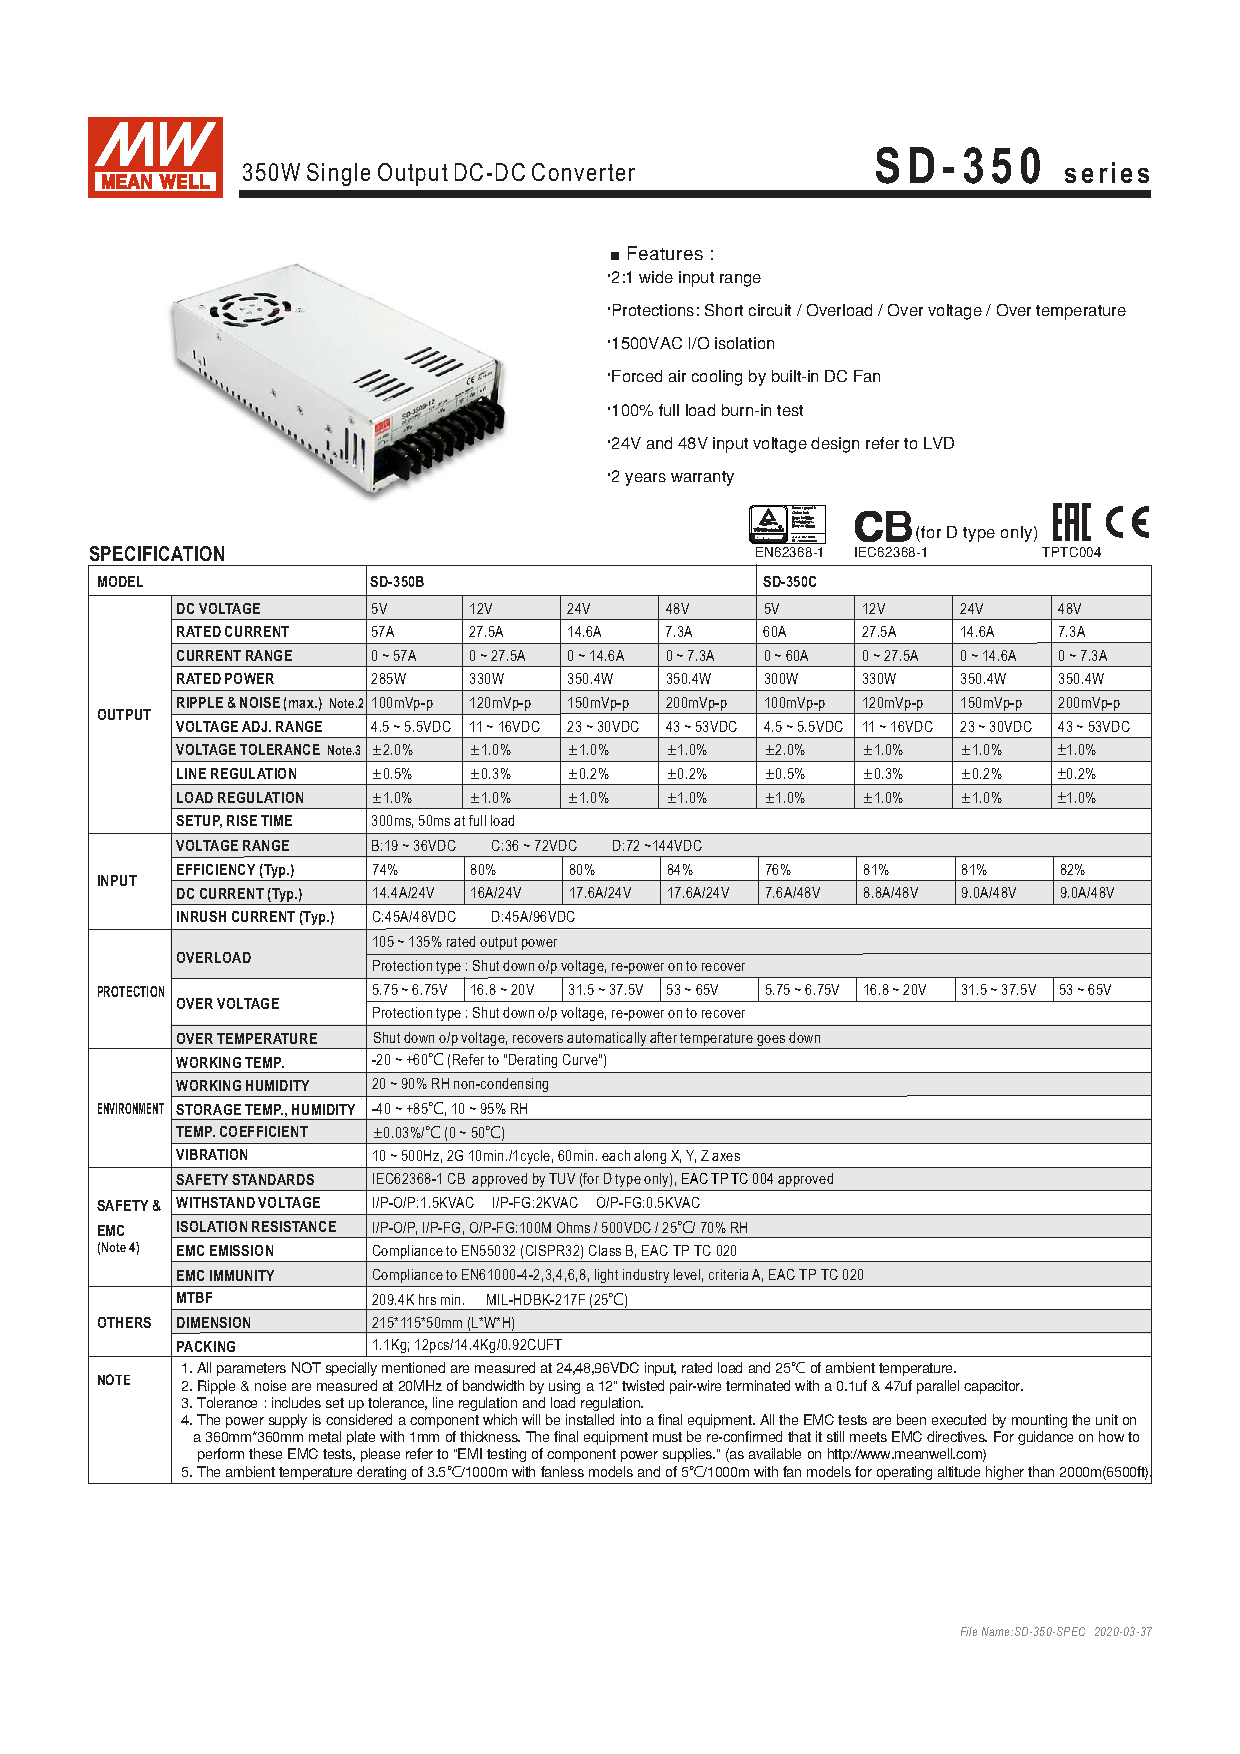
\includepdf[pages=1, pagecommand={\thispagestyle{fancy}}, pagecommand={\subsection{Mean Well SD-350C-12} \label{app:mw12}}, scale=0.8] {pdf/meanwell12.pdf}
\includepdf[pages=2-, pagecommand={\thispagestyle{fancy}}, scale=0.95] {pdf/meanwell12.pdf}


\includepdf[pages=1, pagecommand={\thispagestyle{fancy}}, pagecommand={\subsection{Raspberry Pi 4 Moddel B} \label{app:rasp}}, scale=0.8] {pdf/raspberry.pdf}

\includepdf[pages=2-, pagecommand={\thispagestyle{fancy}}, scale=0.95] {pdf/raspberry.pdf}